% Created 2024-03-05 Tue 09:45
% Intended LaTeX compiler: pdflatex
\documentclass[presentation]{beamer}
\usepackage[utf8]{inputenc}
\usepackage[T1]{fontenc}
\usepackage{graphicx}
\usepackage{longtable}
\usepackage{wrapfig}
\usepackage{rotating}
\usepackage[normalem]{ulem}
\usepackage{amsmath}
\usepackage{amssymb}
\usepackage{capt-of}
\usepackage{hyperref}
\mode<beamer>{\usetheme{Madrid}}
\definecolor{SUred}{rgb}{0.59375, 0, 0.17969} % SU red (primary)
\definecolor{SUblue}{rgb}{0, 0.17578, 0.38281} % SU blue (secondary)
\setbeamercolor{palette primary}{bg=SUred,fg=white}
\setbeamercolor{palette secondary}{bg=SUblue,fg=white}
\setbeamercolor{palette tertiary}{bg=SUblue,fg=white}
\setbeamercolor{palette quaternary}{bg=SUblue,fg=white}
\setbeamercolor{structure}{fg=SUblue} % itemize, enumerate, etc
\setbeamercolor{section in toc}{fg=SUblue} % TOC sections
% Override palette coloring with secondary
\setbeamercolor{subsection in head/foot}{bg=SUblue,fg=white}
\setbeamercolor{date in head/foot}{bg=SUblue,fg=white}
\institute[SU]{Shenandoah University}
\titlegraphic{\includegraphics[width=0.5\textwidth]{\string~/Documents/suLogo/suLogo.pdf}}
\newcommand{\R}{\mathbb{R}}
\usepackage{tikz}
\usetheme{default}
\author{Chase Mathison\thanks{cmathiso@su.edu}}
\date{6 March 2024}
\title{Inverse Trig Functions}
\hypersetup{
 pdfauthor={Chase Mathison},
 pdftitle={Inverse Trig Functions},
 pdfkeywords={},
 pdfsubject={},
 pdfcreator={Emacs 29.1 (Org mode 9.6.7)}, 
 pdflang={English}}
\begin{document}

\maketitle

\section{Announcements}
\label{sec:org71fa7e0}
\begin{frame}[label={sec:org4259e13}]{Announcements}
\begin{enumerate}
\item Homework in MyOpenMath
\item Exam 2 Friday after Spring Break.
\end{enumerate}
\end{frame}

\section{Lecture}
\label{sec:org94b6eb4}
\begin{frame}[label={sec:orgd09d315}]{Inverse Trigonometric Functions}
The main question we want to answer today is this:  What is the angle \(\theta\) in the following right triangle?

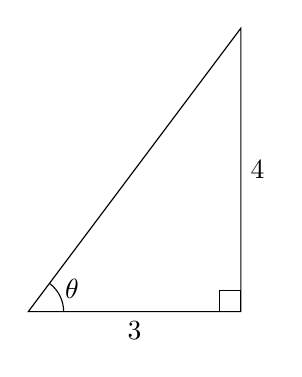
\begin{tikzpicture}[scale=0.9]
  \draw (0,0) -- node[below] {$3$} (3,0) -- node[right] {$4$} (3,4) -- cycle;
  \draw (0.5,0) arc (0:53.13:0.5);
  \node[right] at (40:0.5) {$\theta$};
  \draw (3,0) rectangle ++(-0.3,0.3);
\end{tikzpicture}

Certainly we can find \(\sin(\theta), \cos(\theta)\) and
\(\tan(\theta)\), but how can we say what \(\theta\) is if we know
those values?
\end{frame}

\begin{frame}[label={sec:org43e44c0}]{Let's go to a graph!}
Let's go look at a graph of \(\sin(\theta)\) to see if we can answer
the question on the previous slide.
\end{frame}

\begin{frame}[label={sec:orge2de97e}]{Inverse Functions}
Let's talk about general functions for a second:
\vspace{10in}
\end{frame}

\begin{frame}[label={sec:org9185451}]{The need for restrictions}
So, in order for a function to have an inverse, that function needs to be one-to-one.

Question: Are any of the trig functions one-to-one?

So apparently we need to make a \uline{\hspace*{1in}} on the domain of the
trig functions to turn them into one-to-one functions.  Let's look at
how that's \alert{typically} done.
\end{frame}

\begin{frame}[label={sec:orgda0edb9}]{Desmos!}
\end{frame}

\begin{frame}[label={sec:org42b3977}]{Notation}
The inverse function of the function \(f(x) = \sin(x)\) that has
domain \(\left[ - \frac{\pi}{2},\frac{\pi}{2} \right]\) is the
function \(f^{-1}(x) =\) \uline{\hspace*{1in}}.  This function has a domain
that is identical to the range of \(\sin(x)\).  Similarly, the range
of \(\arcsin(x)\) is the domain of our restricted \(\sin\) function,
so \uline{\hspace*{1in}}.
\end{frame}

\begin{frame}[label={sec:org124b32c}]{Example}
Let's take a second and think how we can restrict the domain of
\(\cos(x)\)to turn it into a one-to-one function.  Then do the same
with \(\tan(x).\)

\vspace{10in}
\end{frame}

\begin{frame}[label={sec:org4385638}]{Example}
Find
\begin{enumerate}
\item \(\arcsin \left( \frac{1}{2} \right)\)
\item \(\arcsin \left( - \frac{\sqrt{2}}{2} \right)\)
\item \(\arccos \left( \frac{1}{2} \right)\)
\item \(\arctan \left( 1 \right)\).
\end{enumerate}

\vspace{10in}
\end{frame}

\begin{frame}[label={sec:org37abc89}]{Example}
Given that \(\sin \left( \frac{\pi}{12} \right) =
\frac{\sqrt{2-\sqrt{3}}}{2},\) write a relation involving inverse
sine.

\vspace{10in}
\end{frame}

\begin{frame}[label={sec:orge6451d1}]{Example}
Now let's see how we can use a calculator to answer the question that we opened class with:

What is the angle \(\theta\) in the following right triangle?

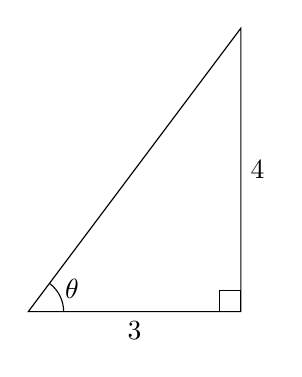
\begin{tikzpicture}[scale=0.9]
  \draw (0,0) -- node[below] {$3$} (3,0) -- node[right] {$4$} (3,4) -- cycle;
  \draw (0.5,0) arc (0:53.13:0.5);
  \node[right] at (40:0.5) {$\theta$};
  \draw (3,0) rectangle ++(-0.3,0.3);
\end{tikzpicture}

\vspace{10in}
\end{frame}
\end{document}